\documentclass[a4paper,12pt]{article}

\usepackage{a4wide}
\usepackage[english]{babel}
\usepackage{hyperref}
\usepackage[utf8]{inputenc}
\usepackage{xspace}
\usepackage{xcolor}
\usepackage{framed}
\usepackage{graphicx}
\usepackage{caption}
\usepackage{subcaption}
\usepackage{float}
\usepackage{array}
\usepackage[compact]{titlesec}

% indentation and paragraph formatting
\usepackage{parskip}
\usepackage{indentfirst}
\setlength{\parskip}{1em}
\setlength{\parindent}{1.1em}

% page style and header/footer
\usepackage{fancyhdr}
\pagestyle{fancy}
\fancyhf{}
\lhead{Machine Learning Competition}
\rhead{Group 15}
\cfoot{--~Page \thepage~--}

\usepackage{titling}
\setlength{\droptitle}{-7em}

\begin{document}

\pagenumbering{gobble}
\title{
\textbf{Machine Learning Competition} \\
\textbf{Group Phase} \\
}
\author{
\textbf{Group 15} \\
Bram De Deyn,
Jan Vermeulen,
Nathan Meheus,
Simone Arena}
\maketitle
\pagenumbering{arabic}

The goal of this competition is creating a machine learning algorithm to optimally predict the ratings for TripAdvisor reviews for hotels. This prediction can be made based on the other elements of the review, i.e. the author, the hotel (price and location), the written text and the date.

\section{Library versions}

We made use of the scikit-learn library, version $0.18$. This made the implementation process much easier, as it provides efficiently implemented methods for all machine learning functionality.
For our doc2vec approach, we made use of gensim, version 0.13.3.

\section{Group interaction and work division}

When the second phase of the competition started, we sat down and studied each other's projects. It became clear that we all focused on a different part and each one of us had something to contribute to a better group project. Putting our areas of expertise together during our weekly meetings led to constantly improving cost values.

\section{Problem/dataset analysis}

The code file \texttt{data\_analysis.py} was used to give us some ideas of the basics of the dataset. Apart from manually inspecting the hotel review files and studying the data representations while debugging the code, this is how most of our data analysis is done. Functions for some basic calculations, information extraction and plots for this report can be found in this file. Resulting histograms or other graphics, can be found in the appendix.

During this analysis we noticed something peculiar. Two authors were responsible for the majority of the reviews, i.e. \texttt{'A TripAdvisor member'} and \texttt{'lass='}. The second one is responsible for the only zero-ratings in the training data set. This is depicted in figure \ref{fig:authorDistr}. In figure \ref{fig:priceDistr}, we can clearly see that there the distribution of the ratings are the same, no matter what the price is. In the end, we only used the features derived from the content.

% insert histograms
\section{Data cleaning}
During the data analysis we noticed that only one user gave zero star ratings and during the analysis of the results, we saw that our models only resulted in a 20\% precision for the zero rating predictions. When creating a review on TripAdvisor, it is also not possible to rate something with zero stars. After a quick discussion, we decided to train the model without the zero star ratings, thus decreasing the amount of classes from 6 to 5. We obtained a score improvement of about $0.03$.

We also tried to add the other components of the reviews as features for our models, but nothing seemed to produce smaller cost values. The features we tried were the length of the written review text, the year of the review, the author, the hotel price, the hotel location, the language of the review content etc. We concluded that the written text of the reviews was the only usable feature.

We started using the confusion matrices to gain detailed information about precisely which predictions were incorrect. That was when we noticed that most of the reviews with zero ratings were predicted with four stars (see Figure \ref{fig:postprocessing-before}). We tried doing some postprocessing to fix these big errors. After some extensive data analysis on these incorrect predictions, we discovered that most of them consist of less than 10\% ASCII characters and have a length between 41 and 52. Our preprocessing consists of predicting a zero rating for the reviews that match these constraints. This resulted in a validation score improvement of $0.03$. Figure \ref{fig:postprocessing-after} depicts the confusion matrix for our predictions with this postprocessing step included.

\begin{figure}[ht!]
    \centering
    \begin{subfigure}[b]{0.48\textwidth}
        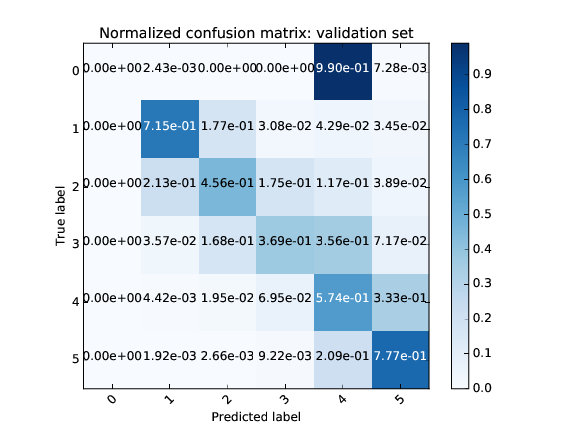
\includegraphics[width=\textwidth]{postprocessing_before.png}
        \caption{Before postprocessing}
        \label{fig:postprocessing-before}
    \end{subfigure}
    ~
    \begin{subfigure}[b]{0.48\textwidth}
        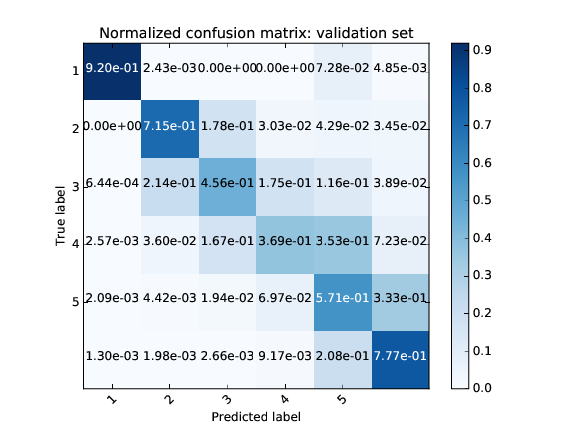
\includegraphics[width=\textwidth]{postprocessing_after.png}
        \caption{After preprocessing}
        \label{fig:postprocessing-after}
    \end{subfigure}
    \caption{Confusion matrices to show the result of our postprocessing step.}
    \label{fig:postprocessing}
\end{figure}

\section{Dimensionality reduction}
At first, the written text of the review (i.e. the actual written text) had to be preprocessed. The content obviously contains the most important features. The preprocessing is done with an intuitive bags of words representation. With the \texttt{TfidfVectorizer} the raw text is converted to a matrix of TF-IDF features, representing how important a word is to a review:\\
\begin{equation}
Word\ importance \sim \frac{Word\ frequency\ in\ all\ reviews\ (Term\ Frequency)}{Average\ word\ frequency\ per\ reviews\ (Document\ frequency)}
\end{equation}

This TF-IDF matrix is then transformed by performing some dimensionality reduction. We keep a certain percentage of the most important features. The dimensionality reduction is based on the ability of the features to discriminate between the different classes [\ref{ref:ordinal}]. We can measure this ability by computing the variance of the set of all ratings corresponding to reviews that contain a certain feature $t_{k}$. A lower variance indicates that a feature is present in only a small number of classes, and is thus a good feature to discriminate a certain class. There is however a caveat, if a feature would only occur in a few reviews, corresponding to the same class, the variance would be low, but it would not be an interesting feature since most of the reviews do not contain this feature. To overcome this, we multiply the variance with the inverse document frequency, to a certain power $a$. We call this product $\sigma$, and sort the features by ascending order, per class for which the feature is the most discriminating, i.o.w. the mean of the previously mentioned set. If we would not sort them per class, we might end up with features that are only able to discriminate one class from all the others.
\begin{equation}
    \sigma = (Var(t_{k})+\epsilon)*IDF(t_{k})^a
\end{equation}
We add $\epsilon$ to the variance to avoid a zero factor, which would result in a $\sigma$-value of 0, without taking the IDF-value into account. This results in three hyperparameters that need to be determined, the $a$-value which accounts for the importance of occurrence, the $\epsilon$-value to avoid zero variances to be wrongly selected as informative, and the percentage of features to keep, also called the reduction level. The code for this can be found in \texttt{preprocessor.py}.

Another dimensionality reduction technique that was explored is LSA (= Truncated SVD). The memory constraints for this approach were very strict, as the technique couldn't handle more than approximately 3000 input features. When executing LSA after the strict feature selection, the validation error surged.

\section{Balancing and scaling}
The training data is really skewed towards higher rating reviews. To overcome this, balancing is a commonly used technique. We chose for a SMOTE over-sampling method to increase the number of training samples with a rating between 1 and 3 [\ref{ref:smote}]. The implementation of this method can be found in  \texttt{balance.py}. It was however never used in an actual submission, since the validation error increased approximately $0.03$ when using balancing.

Balancing is also an option for the LogisticRegression model of scikit-learn. We tested and discussed this below.
% insert plots and more information

Another well known technique in machine learning is scaling the input data (extracting the bias and scaling the the standard deviation to 1). This was also explored in \texttt{balance.py}, but had a negative influence on obtained results.

\section{Machine learning techniques}

\subsection{Combining models of individual phase}

After combining our preprocessing techniques, we compared the score results of our models. This is also shown in the execution results (see Table \ref{tab:ensemble-results}) of \texttt{ensemble.py} (i.e. the ensembles with only one model). Afterwards, we tried a lot of model combinations in a VotingClassifier in \texttt{ensemble.py}, both with hard and soft voting, weighting of classes (i.e. balancing) and not. As LogisticRegression resulted in the best scores during the individual phase, we tried variating the solver (i.e. 'sag' or 'lbfgs'), the class weight (i.e. 'balanced' or not) and multi class options (i.e. the default 'ovr' or 'multinomial'). The 'newton-cg' and 'liblinear' solvers are not used, because they used too much memory resulting in memory errors. The results show the best ensembles and ensembles with parts of it. We reached $0.4127$ as our best validation score.

\begin{table}[]
    \centering
    \begin{tabular}{|>{\centering\arraybackslash} m{3cm} | >{\centering\arraybackslash} m{12cm}|} \hline
    
    \textbf{Score} & \textbf{Model/Ensemble} \\ \hline\hline
    
    0.421121646157 & Logistic Regression (solver: 'sag'); soft/hard voting \\ \hline
    0.447397619528 & Logistic Regression (solver: 'sag' \& balanced); soft voting \\ \hline
    0.421953802703 & Logistic Regression (solver: 'sag \& multinomial classes); soft/hard voting \\ \hline
    0.420995561832 & Logistic Regression (solver: 'lbfgs'); soft/hard voting\\ \hline
    0.447624571313 & Logistic Regression (solver: 'lbfgs' \& balanced) \\ \hline
    0.425484163809 & Logistic Regression (solver: 'lbfgs' \& multinomial classes); soft/hard voting \\ \hline
    0.431687512608 & LinearSVC; hard voting \\ \hline
    0.459678232802 & Multinomial Naive Bayes \\ \hline \hline
    
    0.447246318338 & Logistic Regression (solver: 'sag' \& balanced) \newline Logistic Regression (solver: 'lbfgs' \& balanced) \\ \hline
    0.421096429292 & Logistic Regression (solver: 'sag' \& balanced) \newline Multinomial Naive Bayes; soft voting \\ \hline
    0.418448658463 & Logistic Regression (solver: 'lbfgs' \& balanced) \newline Multinomial Naive Bayes; soft voting \\ \hline
    0.412724430099 & Logistic Regression (solver: 'sag' \& balanced) \newline Logistic Regression (solver: 'lbfgs' \& balanced) \newline Multinomial Naive Bayes; soft voting \\ \hline
    
    \end{tabular}
    \caption{The most important results from \texttt{ensemble.py}. The first part depicts the single models, the second part depicts the ensembles.}
    \label{tab:ensemble-results}
\end{table}

The best ensemble thus consists of two variations of Logistic Regression and a Multinomial Naive Bayes model. The two logistic regression models both have balancing enabled and use the solvers 'sag' and 'lbfgs'. 

\subsection{Doc2vec}
Doc2vec is a 2 layer neural network that represents documents as vectors [\ref{ref:word2vec}]. We used it in two different approaches. In the first approach we transformed all reviews to vectors, constructed the most representative vector per class (this is basically the centre of the featurespace for a certain class), and predicted the ratings by computing the cosine similarity. This way we obtained a mean absolute error of $0.9$.

In the alternative approach, we build a feature matrix from all obtained vector representations, and used this as input for a logistic regression classifier. This resulted in a mean absolute error of approximately $0.7$, which was still a lot worse than the simpler methods used during the individual phase.

\section{Analysis of intermediate results}
To analyse our results, we used functions like \texttt{classification\_report} and \texttt{confusion\_{\allowbreak}matrix} (e.g. Figure \ref{fig:postprocessing}) from \texttt{sklearn.metrics}. This gives us detailed information about the precision and recall of our predictions per rating or class. We used this to determine where we could improve our preprocessing and model, and whether we were over- or underfitting.

We also made a change based on feedback given during one of the feedback lectures. At first, we didn't consider the hotels when we split the training data set in a train and validation set. Doing this split by hotel instead of by review, our validation score became more accurate and was much closer to the scores we received on Kaggle. This is because the test data set contains unique hotels, which are not present in the training data set.

\section{Hyperparameter tuning}
Our approach requires a lot of hyperparameters to be tuned. First of all, the hyperparameters associated with the dimensionality reduction ($a$, $\epsilon$ and the reduction level). And on top of that, the model parameters, for which the combinations grow rapidly when adding models together in an ensemble. We used different approaches to tune these hyperparameters, the best approach would be to test all possible combinations of dimensionality reduction parameters and model parameters. Due to the long run time and high memory requirements, we did this for a fixed validation set. With the obtained parameters for the dimensionality reduction, we did some extra fine tuning for the model parameters with  Shuffle \& Split cross validation. We used Shuffle \& Split cross validation, because it's an easy implementation when the goal is to keep reviews from a certain hotel contained to only the training or only the validation set. The code for all approaches can be found in \texttt{tune\_hyperpar.py}.

The influence of the a-value and the reduction level can be seen on figure \ref{fig:preprop_hyper}, in the appendix. This behaviour is easily explained. With a low a-value, the reduction level (percentage of features to keep) needs to be high to obtain a good mean absolute error. While for a more appropriate a-value makes it possible to keep only the really most informative features.

As previously discussed, we ended up with an ensemble of three classifiers, with a total of 5 hyperparameters to tune (C- and tol-value for each logistic regression classifier, and the $\alpha$-value for the naive Bayes classifier). With a parameter grid, all possible combination were explored for a wide range of values, this is however not easy to visualize. The optimal parameter setting was chosen based on the lowest mean absolute error averaged over the four shuffled splits.

\section{List of references}

\begin{enumerate}
    \item The documentation, user guides and tutorials on the  sci-kit learning website. -- \url{http://scikit-learn.org/stable/documentation.html}
    \item \label{ref:movie-reviews} Predicting Star Ratings of Movie Review Comments, a report for a Stanford University assignment on Machine Learning -- \url{http://cs229.stanford.edu/proj2011/MehtaPhilipScaria-Predicting%20Star%20Ratings%20from%20Movie%20Review%20Comments.pdf}
    \item StackOverflow on scikit-learn, for scikit-learn programming questions -- \url{http://stackoverflow.com/questions/tagged/scikit-learn}
    \item \label{ref:word2vec} Mikolov, Tomas, et al. "Efficient estimation of word representations in vector space." arXiv preprint arXiv:1301.3781 (2013).
    \item \label{ref:smote} The imbalance-learn documentation on SMOTE. -- \url{http://contrib.scikit-learn.org/imbalanced-learn/generated/imblearn.over_sampling.SMOTE.html}
    \item \label{ref:ordinal}Baccianella, Stefano, Andrea Esuli, and Fabrizio Sebastiani. "Feature selection for ordinal text classification." Neural computation 26.3 (2014): 557-591.
\end{enumerate}

\newpage
\section{Appendix}

\begin{figure}[H]
    \center
    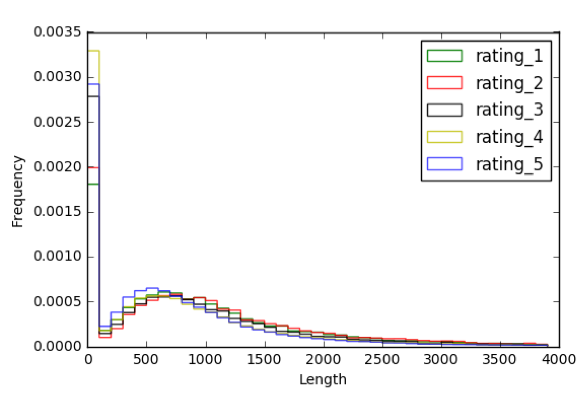
\includegraphics[width=300px]{length_hist.png}
    \caption{Distribution of the content lengths per rating \label{fig:lengthDistr}}
\end{figure}

\begin{figure}[H]
    \center
    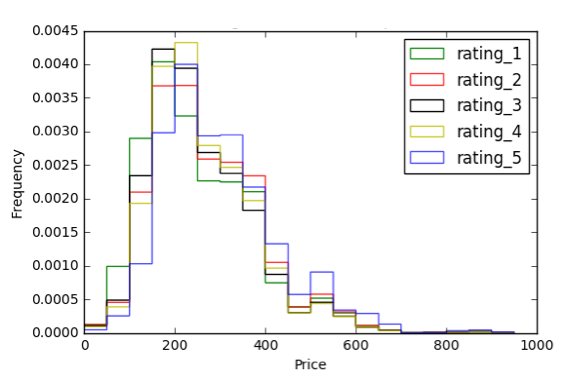
\includegraphics[width=300px]{hotel_hist.png}
    \caption{Distribution of the price per rating \label{fig:priceDistr}}
\end{figure}

\begin{figure}[H]
    \center
    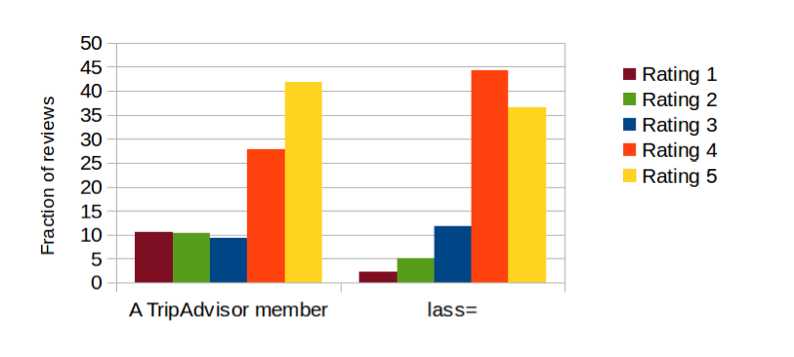
\includegraphics[width=300px]{member_distr.png}
    \caption{Distribution of review authors}
    \label{fig:authorDistr}
\end{figure}

\begin{figure}[H]
    \center
    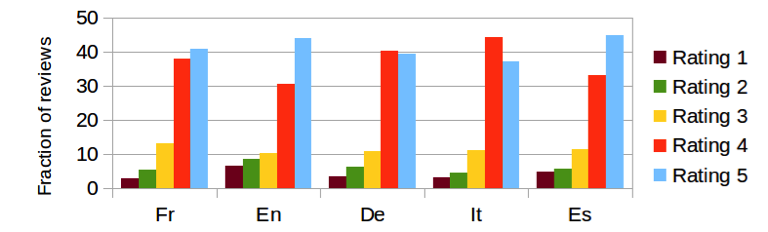
\includegraphics[width=300px]{lang_distr.png}
    \caption{Review language distribution}
    \label{fig:langDistr}
\end{figure}

\begin{figure}[H]
    \center
    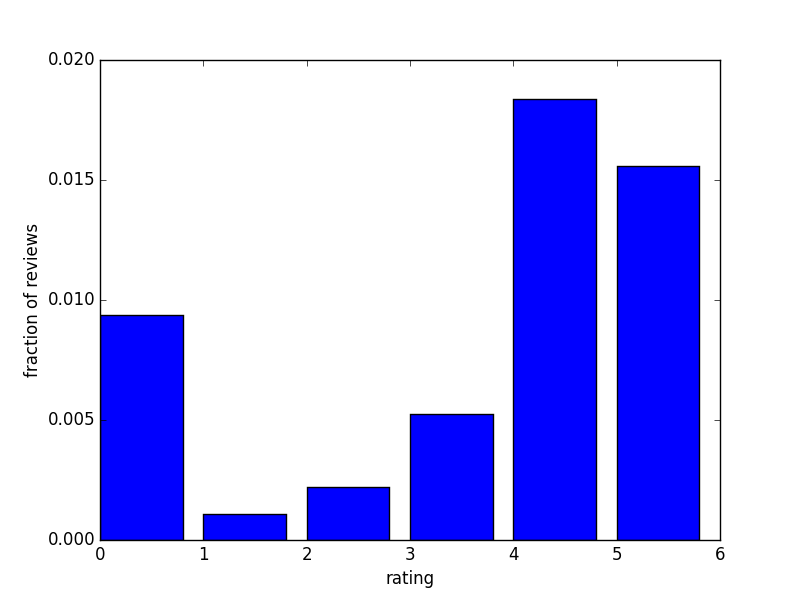
\includegraphics[width=300px]{non-ascii.png}
    \caption{Reviews containing more than 10\% non-ascii chars}
    \label{fig:nonascii}
\end{figure}

\begin{figure}[H]
    \center
    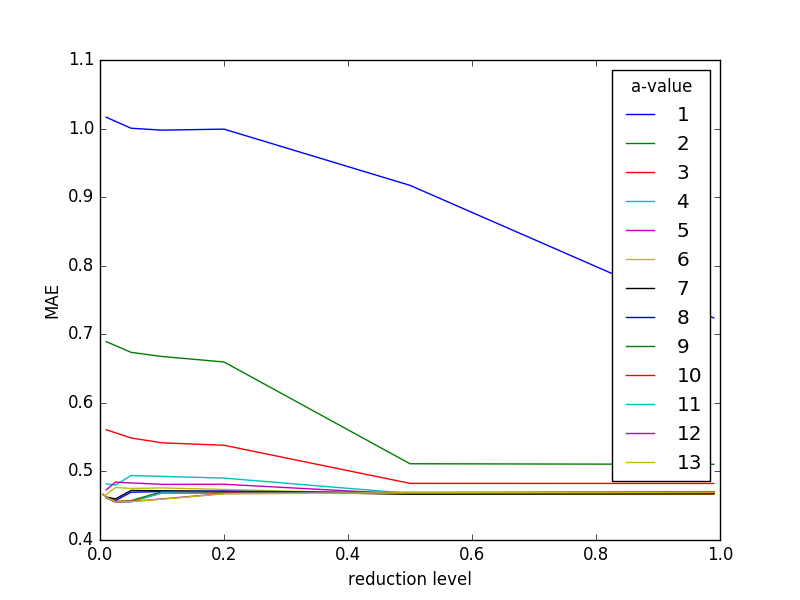
\includegraphics[width=300px]{mae_a_redlevel.png}
    \caption{The effects of the amount of kept features vs the mean absolute error, for different a-values}
    \label{fig:preprop_hyper}
\end{figure}


\end{document}
